\section{Введение} % (fold)

С развитием вычислительных систем и ростом в них доли
программной составляющей, сложность разрабатываемых программ постоянно
возрастает. Также, вследствие большой конкуренции на рынке программного
обеспечения, разработчики вынуждены постоянно снижать сроки разработки новых
версий ПО. Эти факторы неизбежно ведут к снижению качества выпускаемых
продуктов.

Падение уровня качества является проблемой, особенно если программное
обеспечение задействовано в критически важных сферах человеческой деятельности,
например медицине и космонавтике. Поэтому задача повышения качества является
одной из самых актуальных в сфере информационных технологий.

\subsection{Понятие качества} % (fold)

Качество ПО - достаточно абстрактное понятие. Многие понимают под ним, например,
ПО, которое не содержит ошибок. Однако, это лишь одна из характеристик качества.
В стандарте ISO 8402:1994 ``Quality management and quality assurance'' дается
следующее определение качества:

\textbf{Качество программного обеспечения} - это совокупность характеристик ПО,
относящихся к его способности удовлетворять установленные и предполагаемые
потребности.

На данный момент наиболее распространена и используется многоуровневая модель
качества программного обеспечения, представленная в наборе стандартов ISO 9126.
На верхнем уровне выделено 6 основных характеристик качества ПО, каждую из
которых определяют набором атрибутов, имеющих соответствующие метрики для
последующей оценки:

\begin{figure}[h!]
    \begin{center}
        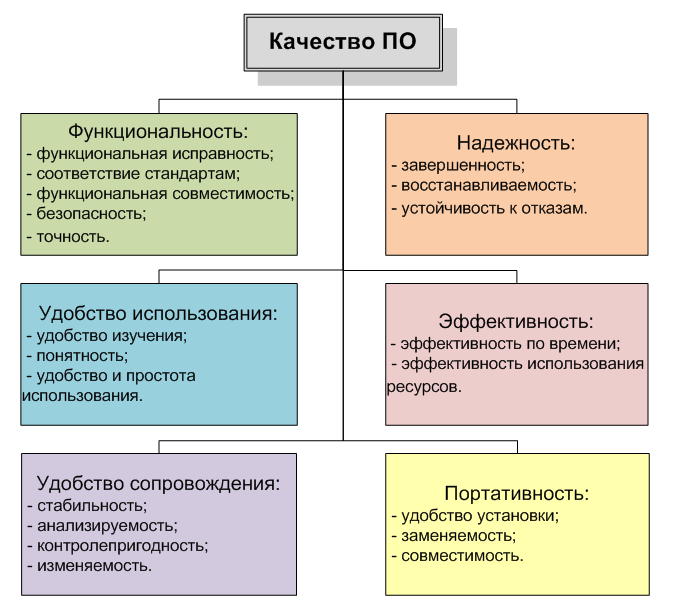
\includegraphics[]{img/quality_chars_iso.png}
    \end{center}
    \caption{Модель качества программного обеспечения}
    \label{fig:figure1}
\end{figure}

\subsection{Верификация и валидация} % (fold)

Верификация и валидация являются видами деятельности, направленными на контроль
качества программного обеспечения и обнаружение ошибок в нем.

\textbf{Верификация} проверяет соответствие одних создаваемых в ходе разработки
и сопровождения ПО артефактов другим, ранее созданным или используемым в
качестве исходных данных, а также соответствие этих артефактов и процессов их
разработки правилам и стандартам.

\textbf{Валидация} проверяет соответствие любых создаваемых или используемых в
ходе разработки и сопровождения ПО артефактов нуждам и потребностям
пользователей и заказчиков этого ПО, с учетом законов предметной области и
ограничений контекста использования ПО.

На рис~\ref{fig:figure2} приведено различие между верификацией и валидацией.

\begin{figure}[h!]
    \begin{center}
        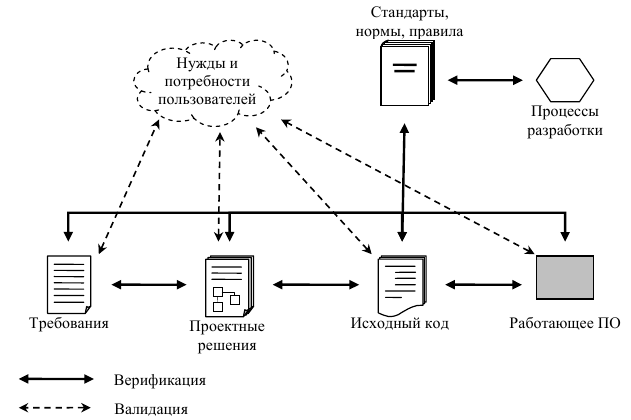
\includegraphics[width=\textwidth]{img/validation_and_verification.png}
    \end{center}
    \caption{Соотношение верификации и валидации}
    \label{fig:figure2}
\end{figure}

\subsection{Задачи верификации} % (fold)

Верификация решает следующие задачи в процессе разработки ПО:

\begin{itemize}
    \item Выявление дефектов различных артефактов разработки ПО.
    \item Выявление критичных и наиболее подверженных ошибкам частей
    создаваемой или сопровождаемой системы.
    \item Контроль и оценка качества ПО.
    \item Предоставление всем заинтересованным лицам информации о текущем
    состоянии проекта и характеристиках его результатов.
    \item Предоставление руководству проекта и разработчикам информации
    для планирования дальнейших работ, а также для принятия решений о
    продолжении проекта, его прекращении или передаче результатов заказчику.
\end{itemize}
